\documentclass[../main.tex]{report}

\begin{document}
    \label{sec:test1}
    
\subsection{Approche probabiliste}
Soient $E_n := \left\{ k \in \mathbb{N}^* ~|~k < n \right\}$ l'ensemble des entiers inférieurs à $n$, $ P_n := \{k \in E_n~|~ k$ est premier$ \}$ l'ensemble des nombres premiers inférieurs à $n$, et la fonction $\pi (n) := \#P_n$, le nombres de premiers inferieurs à $n$.

On a vu que la fonction Li$(x) = \int_2^x \frac{dt}{\log t}$ 
donne une bonne approximation de $\pi(x)$.

Cette fonction peut être approximée par la somme de Riemann de pas constant égal à 1.
\begin{equation}
\label{eq:SommeDeRiemann}
S \left({\frac{1}{\log x}} \right)
= \sum_{k=0}^{n-1} \frac{1}{\log(2 + k)}
= \frac{1}{\log 2} + \sum_{k=3}^{n-1} \frac{1}{\log k}
\end{equation}


La fonction $x \mapsto \frac{1}{\log x}$ est une fonction continue, décroissante et positive sur l'interval $\left[2, \infty \right[$. 
L'erreur entre Li$(x)$ et la fonction en escalier ci-dessus est donc bornée. 
 \[ 
\left| S(\frac{1}{\log x}) - Li(x) \right|
\leq \left| \sum_{k=2}^{n-1} \frac{1}{\log k} - \frac{1}{\log (k+1)} \right| 
 %= \left| \frac{1}{\log (n+1)} - \frac{1}{\log 2} \right|
 = \frac{1}{\log (2)} - \frac{1}{\log (n)}
 < \frac{1}{\log 2}
 < 2
 \]


\subsubsection{Ensembles aléatoires} 

Nous allons utiliser (\ref{eq:SommeDeRiemann}) pour générer des ensembles aléatoires $R_{k} \subset \mathbb{N}, k \in \{1,...,100\}$, de sorte que chaque entier $n$ ait une probabilité de $1/\log(n)$ d'appartenir à l'ensemble. 
\[
\forall~i \in \mathbb{N}, P(i \in R_{k}) = 
\left\{ 
    \begin{array}{cl}
         0 & \mbox{si}~i = 1 \\
         1 & \mbox{si}~i = 2 \\
         \frac{1}{\log i} & \mbox{si}~i \geq 3
    \end{array}
\right.
\]
Ces ensembles seront construits jusqu'à $i = 10^7$: on a donc $R_k \subset \{1,...,10^7\}$. 

Il est à noter deux cas particuliers:
\begin{itemize} 
    \item Le nombre 1 est exclu. En effet, $\frac{1}{\log 1}$ n'est pas défini. Par définition, $1$ n'est pas un nombre premier.
    \item Le nombre 2 est inclus par défaut. En effet, $P(2 \in R_k) = 1$ car $\frac{1}{\log 2} > 1$. De plus, le nombre 2 est par définition, un nombre premier.
\end{itemize}


La fonction $\sigma_{R_k}(n) := \# \{i \in R_{k} | i < n\}$ mesure donc la taille des ensembles jusqu'à un certain $n$. 
Cette fonction est donc une variable aléatoire strictement inférieure à $n$ 
dont l'espérance, que nous noterons $\sigma_R(n)$, est donnée par:
\[ 
\sigma_R(n) = 
\sum_{i=1}^{n-1} 1 \cdot P(i \in R_k) 
= 1 + \sum_{i=3}^{n-1} \frac{1}{\log i}
\]
%\begin{equation}
%\label{eq:esperance}
%E[\sigma_{R_k}(n)]
%= \sum_{k=1}^{n-1} P(k \in R_k)
%= 0 + 1 + \frac{1}{\log 3} + ... + \frac{1}{\log (n-1)}
%= 1 + \sum_{k=3}^{n-1} \frac{1}{\log k}
%\end{equation}

%Notons $\sigma_R(n)$ l'ésperance de cette variable aléatoire.
L'erreur entre $\sigma_R(n)$ et la somme de Riemann (\ref{eq:SommeDeRiemann}) est constante, égale à
$\frac{1}{\log 2}- 1 < 1$.

Les ensembles aléatoires générés de cette manière suivront donc une distribution similaire à Li$(x)$, et donc à $\pi(x)$
(voir figures \ref{fig:comparison_sigma_prob} et \ref{fig:prob_sample}).

\begin{figure}[H]
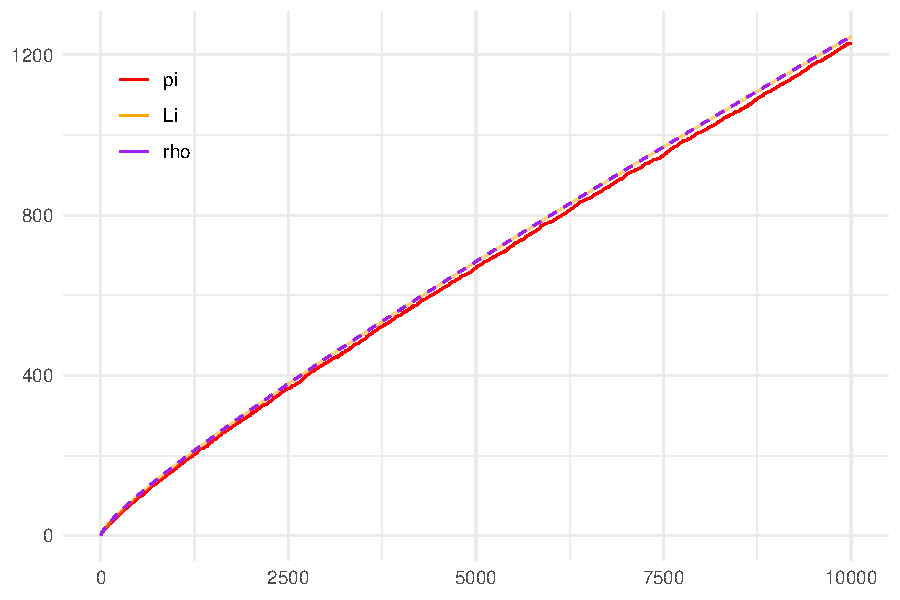
\includegraphics[width=\textwidth]{comparison_sigma_prob}
\caption{Graphes des fonctions $\pi$, Li and $\sigma_R$. Li et $\sigma_R$ sont superposées.}
\label{fig:comparison_sigma_prob}
\end{figure}

\begin{figure}[H]
	\centering
	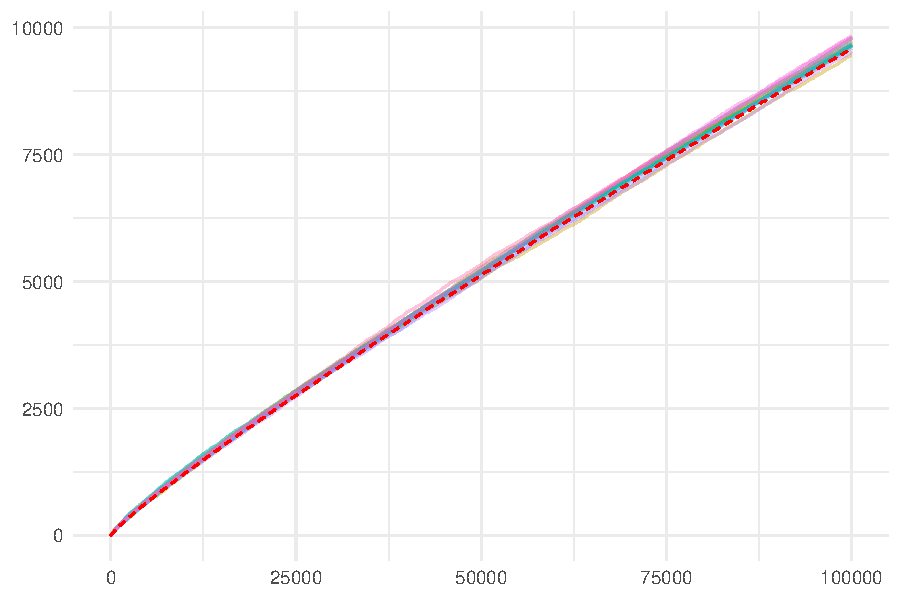
\includegraphics[width=\textwidth]{prob_samples}
	\caption{graphes des fonctions $\sigma_{R_k}$ pour $k \leq 25$ (i.e. les 25 premiers ensembles) et $\pi$ (en pointillé)}
	\label{fig:prob_sample}
\end{figure}
\end{document}
